\begin{center}
\scalebox{0.6}{
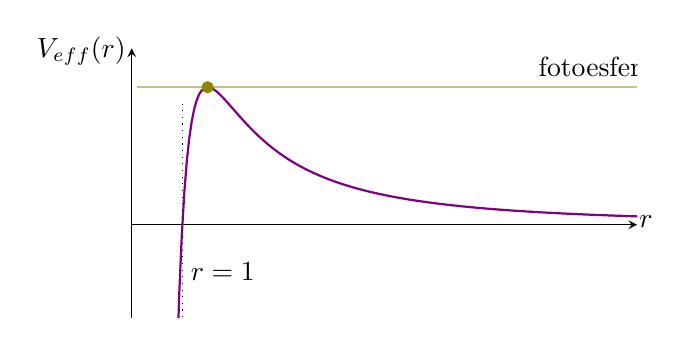
\begin{tikzpicture}
\begin{axis}[
    width=8cm,
    height=5cm,
    axis lines=middle,
    ticks=none,
    xlabel={$r$},
    ylabel={$V_{\text{eff}}(r)$},
    domain=0.2:10,
    samples=200,
    ymin=-0.1,  % mantener parte negativa
    ymax=0.19,   % recortado arriba para centrarse en lo relevante
    xmin=0,
    xmax=10,
    ylabel style={at={(axis description cs:-0.10,0.9)}, anchor=south},
    xlabel style={at={(axis description cs:1.05,0.3)},}
]

% Potencial efectivo
\addplot[violet, thick, restrict y to domain=-5:0.19] {(1/(x^2)) - (1/x^3)};

% Línea vertical punteada
\addplot[dotted, thin] coordinates {(1,-0.3) (1,0.13)};
\node at (axis cs:1.8,-0.05) {$r=1$};

% Línea naranja (fotoesfera)
\addplot[olive, thick, opacity=0.5, domain=0.1:10] {4/27};
\node at (axis cs:9.2,0.17) {fotoesfera};

\addplot[only marks, mark=*, olive] coordinates {(3/2,4/27)};

\end{axis}
\end{tikzpicture}
}
\end{center}
